\section{Nonlinear product validation with known covariance}
\label{sec:product-validation}
The software product is tested separately from the preceding
54-observable theory experiment. Its ordinary compact-lens inference fits
mass, reference center and observer proper motion, two shear components,
and two free source coordinates at every row. Distances, redshifts and the
absolute astrometric frame are supplied calibrations. The baseline
validation is entirely synthetic; its adopted errors do not specify an
instrument capability. Optional R1 information retains the separate
conditional-exterior and physical-amplitude restrictions.
The frozen nearby fixture contains a $10^5 M_\odot$ lens at $D_l=1$ Mpc,
three background source positions sampled at each of three epochs over
ten observer years, and true motion $(0.065,-0.038)$ mas/yr.
The nine rows supply 54 image-coordinate, log-flux-ratio and delay
measurements. Their declared base noise scales are $0.02$ mas, $0.005$ and
$3\times10^{-4}$ s, respectively, with supplied astrometric and timing
correlations. The full covariance $C$ is retained in
$\chi^2=(d-f)^T C^{-1}(d-f)$; errors are not rescaled by the fitted
reduced $\chi^2$. These inputs test a resolved primary-pair model with
free source positions, rather than assume a known unlensed source track.

\begin{figure}[tbp]
\centering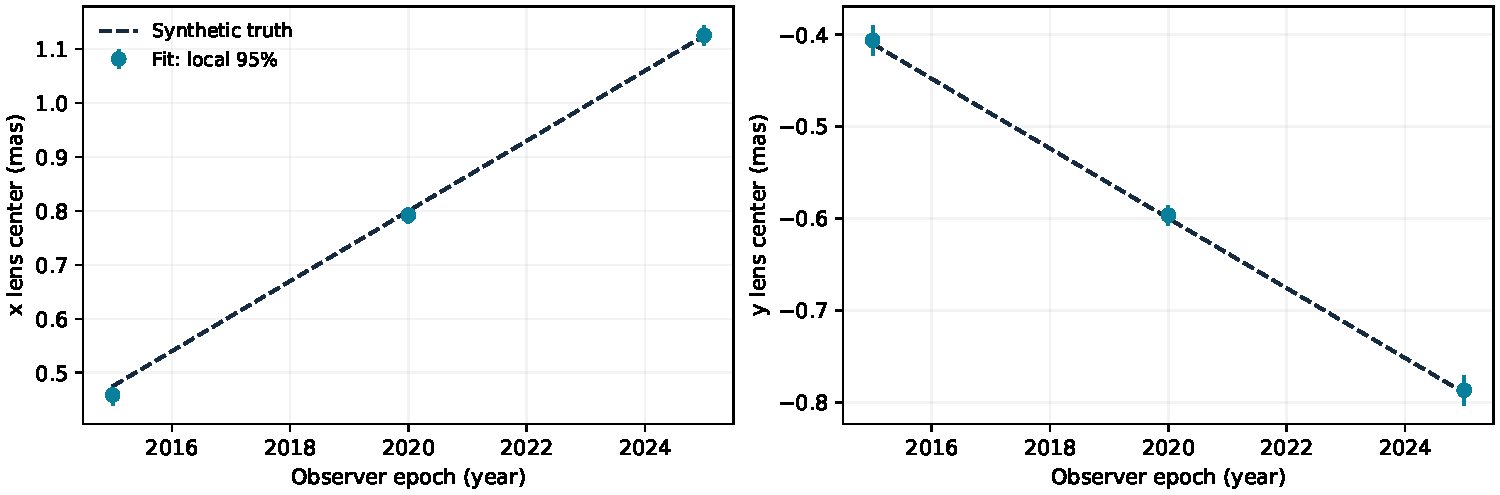
\includegraphics[width=\linewidth]{../figures/product_track.pdf}
\caption{The noisy nearby synthetic fixture: recovered lens-center
coordinates with local 95\% marginal intervals propagated from the full
center--motion covariance, against truth used only for scoring.
Repeated rows at each epoch overlap. This is a ten-year three-source
product test, distinct from the broad single-track information scan.}
\label{fig:product-track}
\end{figure}

The noiseless recovery control (C6) uses the data-derived initializer and
two fixed perturbations, including mass factors 1.5 and 0.65 and shifts
of center, motion, sources and shear. Each fit uses three internal starts.
All recover the mass, center and motion within the frozen relative or
reference-scale tolerances $10^{-5}$; the largest $\chi^2$ is
$3.01\times10^{-23}$, below the fixed $10^{-6}$ criterion. Truth is used
to score recovery, not supplied as an initializer. This checks nonlinear
solver recovery for this fixture, not global likelihood uniqueness.

\subsection{A fixed repeated-noise calibration}
Control C7 draws 64 independent Gaussian noise vectors using the full
$C$, a single frozen PCG64 stream seeded 4932026, and one start per
ordinary-lens fit with shear admitted. Every realization remains in the
record and coverage denominator; an exception, rejected fit or unavailable
interval would count as a miss. All 64 fits converge and return the
product's \texttt{TRACKED} status, with no excluded failures.
The reported intervals are local known-covariance Gaussian intervals,
not reoptimized likelihood profiles. For mass we use
$\widehat M\exp[\pm1.959964\,\sigma_M/\widehat M]$; center and motion
use $\widehat\theta\pm1.959964\,\sigma_\theta$.

\begin{table}[tbp]
\centering\small
\caption{Frozen 64-draw local 95\% interval coverage. Each exact two-sided
binomial test has null coverage 0.95 and rejection level $\alpha=0.01$.
All five tests are reported without a multiple-testing adjustment.}
\label{tab:product-coverage}
\begin{tabular}{@{}lrrr@{}}
\toprule
Coordinate & Covered / 64 & Fraction & Exact $p$\\
\midrule
Mass $M$ & 61 & 0.9531 & 1.0000\\
Center $x$ & 59 & 0.9219 & 0.2532\\
Center $y$ & 61 & 0.9531 & 1.0000\\
Motion $x$ & 61 & 0.9531 & 1.0000\\
Motion $y$ & 61 & 0.9531 & 1.0000\\
\bottomrule
\end{tabular}
\end{table}

None fails the preregistered gross-miscalibration guard
(Table~\ref{tab:product-coverage}). The exact 95\% binomial interval for
61/64 coverage is $[0.8691,0.9902]$, and for 59/64 it is
$[0.8270,0.9741]$: 64 draws provide a limited calibration check.
The receipt also retains parameter bias and scatter. In particular, the
mean $y$-motion error is $3.98\times10^{-4}$ mas/yr, about 2.75 estimated
standard errors of its ensemble mean. Passing the frozen coverage test
does not establish negligible bias or universal coverage.

\subsection{Weak information, model mismatch and finite cause ambiguity}
The negative controls preserve unsuccessful scientific outcomes
(Table~\ref{tab:product-controls}). The ten-year cosmological fixture
(C8) has true motion $(5,-3)\times10^{-5}$ mas/yr and returns
\texttt{PARTIALLY\_IDENTIFIED}, with motion signal-to-noise 0.00482 and
component errors $(0.0121,0.0124)$ mas/yr. Its mass information does not
license a resolved motion claim. For a separate conventional-shear
fixture (C11), omitting shear gives a rejected fit at the frozen
goodness-of-fit criterion $p<0.001$; admitting shear recovers the declared
$(0.03,-0.018)$ coefficients. Residual structure is therefore not assigned
automatically to an R1 envelope or a new physical cause.

\begin{table}[tbp]
\centering\small
\caption{Controls with scientifically meaningful weak or null outcomes.}
\label{tab:product-controls}
\begin{tabular}{@{}lll@{}}
\toprule
Control & Quantity & Outcome\\
\midrule
C8: short cosmological track & Motion SNR $0.00482$ & Unresolved motion\\
C11: shear omitted & $\chi^2=28297.8$ & Fit rejected\\
C11: shear admitted & $\chi^2=1.95\times10^{-22}$ & Baseline recovered\\
C9: harmonic / compact pair & Four columns, rank two & Two exact nulls\\
\bottomrule
\end{tabular}
\end{table}

For C9 the zero-flux harmonic boundary response is exactly an ordinary
compact $r^{-2}$ quadrupole, with coefficient
$-\widehat\beta N_2 r_0^3/[3m_{\rm ref}(r_E^{\rm ref})^2]$ per boundary
amplitude, in the declared reference lens units.
Three finite operator comparisons and compensating coefficient changes
agree in potential, gradient and Hessian to $2.22\times10^{-16}$.
Four combined compact/boundary columns have rank two. Large formal
coefficients are confined to this operator identity test; public
prediction separately rejects that nonadmitted state. They are not
enlarged physical signals. The current nonlinear fit does not expose a
joint free fit of both degenerate amplitude pairs, so separate-amplitude
interval calibration is not claimed.
These controls accompany the released independent interface, physical-unit,
covariance and admission tests. Versioned JSON receipts retain every
draw, initializer, criterion, runtime and SHA-256 source hash; the R1
provider inputs are pinned and checked on loading. The scripts
\texttt{calibrate\_product.py} and
\texttt{check\_finite\_harmonic\_degeneracy.py} reproduce the controls.
The validated scope is the declared synthetic compact-lens families and
local intervals. Unknown calibration, broader environmental freedom,
critical image configurations, observational sensitivity and horizon
identification remain outside this validation.
